\documentclass[preprint,authoryear]{elsarticle}

\usepackage{lineno}
\usepackage{graphicx}
\usepackage{amsmath}
\usepackage{hyperref}
\usepackage{booktabs}
\usepackage{xcolor}
\usepackage{subcaption}

\journal{Antiviral Research}

% Evidence-grading color scheme
\newcommand{\strongclaim}[1]{\textcolor{green!60!black}{#1}}
\newcommand{\moderateclaim}[1]{\textcolor{orange}{#1}}
\newcommand{\hypothesisclaim}[1]{\textcolor{red}{#1}}
\newcommand{\claimlabel}[1]{\textbf{[#1]}}

\begin{document}

\begin{frontmatter}

\title{Under current compiled phenotypic evidence, HIV-1 lenacapavir resistance is driven primarily by mutation identity, whereas subtype adds little explanatory value}

\author[inst1,inst2]{Yiheng Yang\corref{cor1}}
\cortext[cor1]{Corresponding author}
\ead{yangyiheng@mail.dlut.edu.cn}

\address[inst1]{School of Future Technology, Dalian University of Technology, Dalian, China}
\address[inst2]{School of Bioengineering, Dalian University of Technology, Dalian, China}

\begin{abstract}
\textbf{Background}: Lenacapavir (LEN) resistance interpretation requires deciding whether phenotype is explained primarily by mutation identity or by subtype-level context. 
\textbf{Methods}: Following PRISMA 2020, we screened 87 records and included 11 studies (26 quantitative observations, 16 mutations). We harmonized fold-change data on the log$_{10}$ scale and compared four model levels (M0--M3), with bootstrap ranking stability (n=1,000), leave-one-study-out validation, and supportive epistasis, structural, and conservation analyses.
\textbf{Results}: M1 (mutation-only) was the best-supported model (AIC=40.9, R$^{2}$=0.946). Adding subtype (M2) provided little additional explanatory value at current data depth ($\sigma^2=0.000000$ boundary convergence). Top mutation rankings were stable (N57H rank 1.0 $\pm$ 0.0; M66I rank 1.9 $\pm$ 0.4). N57H (4,890-fold) and M66I (3,200-fold) showed the highest single-mutation resistance. Combination analysis showed Q67H+N74D positive synergy (150-fold observed vs 25-fold additive expectation), Q67H+K70R context-sensitive variability (76-fold range), and putative compensatory patterns for M66I+A105T (111-fold) and M66I+T107A (234-fold). Structural perturbation scores correlated with phenotype (r=0.886, $p$=0.003), and LEN-contact residues were highly conserved (median=0.97).
\textbf{Conclusions}: Under current compiled phenotypic evidence, LEN resistance is driven primarily by mutation identity, while subtype contributes little additional explanatory value at the present data level. This supports mutation-first surveillance triage and prioritizes next-step subtype-stratified phenotyping.
\end{abstract}

\begin{keyword}
HIV-1 \sep Lenacapavir \sep Capsid inhibitor \sep Drug resistance \sep Evidence synthesis \sep Model comparison \sep Epistasis \sep Surveillance
\end{keyword}

\end{frontmatter}

\linenumbers

%============================================================
\section{Introduction}
%============================================================

Lenacapavir (LEN), a first-in-class HIV-1 capsid inhibitor, has introduced a long-acting treatment paradigm with twice-yearly dosing and potent activity in heavily treatment-experienced populations \cite{Link2020,Segal2022}. As LEN use expands across treatment and prevention contexts, resistance interpretation becomes a surveillance-critical task rather than a purely descriptive cataloging exercise.

Resistance-associated mutations (RAMs) cluster around two structural interfaces of the capsid hexamer, including the hydrophobic pocket (L56V, N57H, M66I, Q67H) and the NTD-CTD interface (N74D, K70R, K70N) \cite{Bester2022,Margot2025}. The central scientific question is whether LEN resistance should be interpreted primarily at the mutation level or whether viral background, including subtype, substantially modulates those mutation-level effects in ways that alter interpretation and triage.

Existing studies and compilations have substantially expanded the list of LEN-associated phenotypes \cite{Hansen2025}, but the key inferential gap remains: relative explanatory contribution from mutation-level versus subtype-level terms has not been explicitly quantified as a level-of-explanation comparison under sparse evidence. A common over-interpretation follows from this gap: near-zero subtype variance in small, imbalanced datasets is sometimes read as evidence that subtype effects are absent, although this conclusion exceeds what the data can support.

Here, we systematically synthesize published phenotypic evidence to determine which interpretation is best supported by current data, to quantify how much explanatory value subtype adds beyond mutation identity, and to translate that distinction into a surveillance-oriented evidence framework. Rather than seeking maximal certainty from limited data, we prioritize a boundary-aware interpretation that is explicit about what can be stated now and what still requires targeted subtype-stratified evidence generation.

%============================================================
\section{Materials and Methods}
%============================================================

\subsection{Evidence Synthesis (PRISMA 2020)}

We followed PRISMA 2020 reporting guidelines \cite{Page2021} to make the evidence boundary auditable before downstream modeling. A systematic literature search was conducted in PubMed using terms: (lenacapavir OR GS-6207) AND (resistance OR capsid OR mutation OR fold-change). Identification: 82 PubMed records + 5 additional sources = 87 total. After deduplication ($n=78$), title/abstract screening excluded 56 records. Full-text review of 22 records excluded 11 (8 lacking quantitative data; 3 HIV-2 only). Eleven studies provided 26 quantitative fold-change observations meeting inclusion criteria (Figure~\ref{fig:evidence}).

\textbf{Inclusion criteria}: (1) Quantitative phenotypic resistance measurement (fold-change vs wild-type); (2) HIV-1 only; (3) Peer-reviewed publication or clinical trial report; (4) Identified resistance mutation(s). \textbf{Exclusion}: HIV-2, qualitative only, review articles.

\subsection{Data Harmonization}

To avoid direct comparison of non-commensurate assay outputs, all fold-change (FC) values were harmonized to log$_{10}$ scale:
\begin{equation}
\text{log}_{10}\text{FC} = \log_{10}\left(\frac{\text{EC}_{50,\text{mutant}}}{\text{EC}_{50,\text{WT}}}\right)
\end{equation}
Each observation received: (1) \textit{context tier} (clinical $>$ in vitro $>$ natural polymorphism); (2) \textit{quality score} (1--3 based on experimental rigor); (3) \textit{unique observation ID} with full provenance. All data and code are available in the project repository.

\subsection{Model Comparison Framework}

To compare explanatory levels rather than maximize prediction complexity, we fit four nested models using ordinary least squares with dummy-coded mutation effects:
\begin{align}
\text{M0 (intercept):} &\quad \log_{10}\text{FC} = \beta_0 + \epsilon \\
\text{M1 (mutation):} &\quad \log_{10}\text{FC} = \beta_0 + \sum_k \beta_k \cdot \mathbf{1}[\text{mut}_k] + \epsilon \\
\text{M2 (mut + subtype):} &\quad \log_{10}\text{FC} = \beta_0 + \sum_k \beta_k \cdot \mathbf{1}[\text{mut}_k] + u_j + \epsilon, \\
&\quad u_j \sim N(0, \sigma^2) \\
\text{M3 (mut + study):} &\quad \log_{10}\text{FC} = \beta_0 + \sum_k \beta_k \cdot \mathbf{1}[\text{mut}_k] + v_s + \epsilon, \\
&\quad v_s \sim N(0, \tau^2)
\end{align}

AIC and BIC were computed for model comparison. Leave-one-study-out (LOSO) cross-validation was performed ($n=11$ folds, RMSE and MAE reported) to test robustness against study-level removal rather than claim broad generalizability. Bootstrap ranking stability was assessed with 1,000 resamplings (with replacement); per-mutation rank mean and standard deviation were calculated.

\subsection{Epistasis Analysis}

To interpret combinations without overstating sparse pairwise evidence, double mutants were benchmarked against additive expectations under independence in log space:
\begin{equation}
\log_{10}\text{FC}_{\text{expected}} = \log_{10}\text{FC}_{\text{mut1}} + \log_{10}\text{FC}_{\text{mut2}}
\end{equation}

Epistatic residual $= \log_{10}\text{FC}_{\text{observed}} - \log_{10}\text{FC}_{\text{expected}}$. Positive residuals indicate positive synergy (greater than additive); negative residuals indicate compensation (less than additive). Single mutant reference values were taken from the same study when available, otherwise from pooled means.

\subsection{Structural Perturbation Analysis}

Structural analysis was used as a supportive mechanistic line, not as a standalone proof of causal hierarchy. Published structural data from Bester et al. \cite{Bester2022} (PDB: 6VKV, 7RAO) were used to derive perturbation metrics for 8 mutations: H-bond losses, estimated steric clash score, binding $\Delta\Delta G$ (published FoldX values), and CA-contact count changes. A composite perturbation score was calculated as a weighted sum. Pearson correlation between perturbation score and log$_{10}$FC was computed.

\subsection{Sequence Conservation Analysis}

Evolutionary analysis was used to contextualize mutation-level interpretation under background diversity constraints. Conservation scores for 13 LEN-contact residues were compiled from published literature (mBio 2022, FDA prescribing information, Los Alamos HIV Sequence Database) \cite{Bester2022,FDA2025,LANL2025}. Shannon entropy was computed where sufficient subtype-stratified frequency data were available. Natural polymorphism prevalences were extracted from published population-level surveys.

\subsection{Claim Grading}

Claim grading was predefined to constrain inference strength and prevent overextension from sparse evidence:
\begin{itemize}
  \item \claimlabel{S} \textbf{Strong}: Supported by multiple independent observations ($n \geq 5$), stable across bootstrap resampling, consistent across context tiers.
  \item \claimlabel{M} \textbf{Moderate}: Supported by $n=2$--4 observations or a single study with quantitative analysis; directionally consistent but not independently replicated.
  \item \claimlabel{H} \textbf{Hypothesis-generating}: Based on $n \leq 2$ observations, indirect evidence, or mechanistic inference; requires targeted validation.
\end{itemize}

%============================================================
\section{Results}
%============================================================

\subsection{Evidence Landscape Defines the Inference Boundary}

\begin{figure*}[!t]
\centering
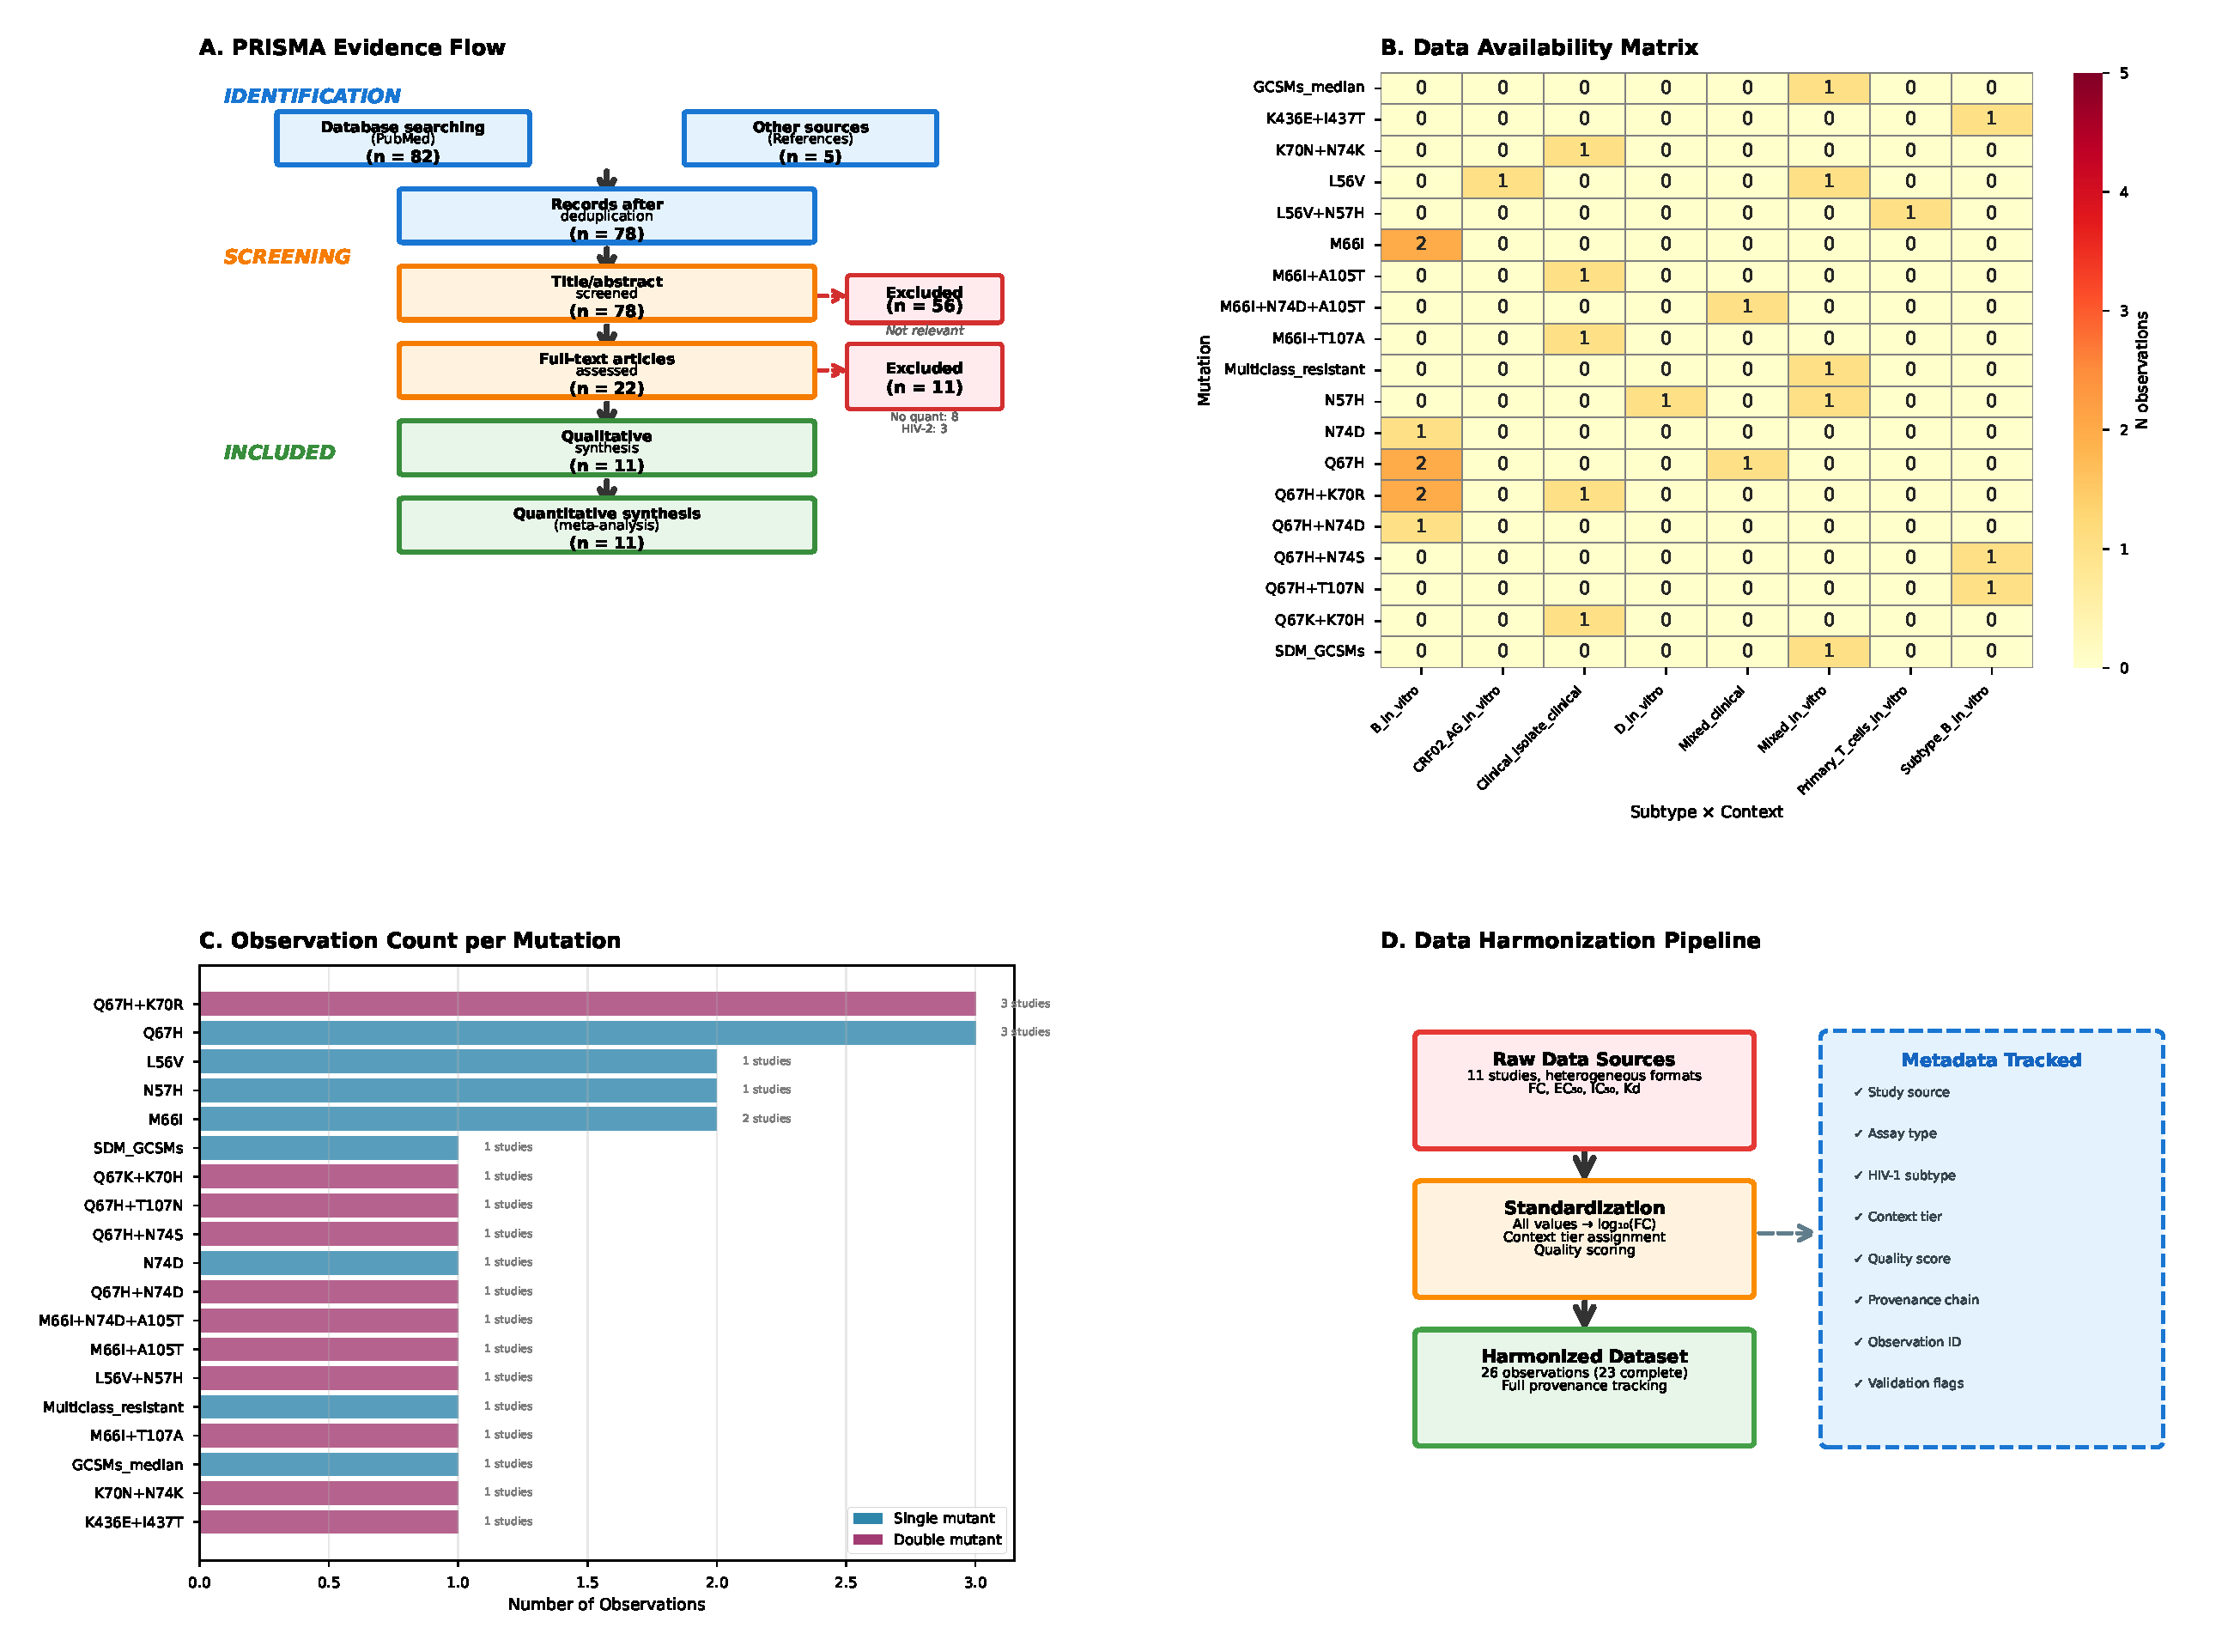
\includegraphics[width=0.95\textwidth,keepaspectratio]{figure1_evidence_landscape.pdf}
\caption{\textbf{Evidence landscape.}
\textbf{(A)} PRISMA 2020 flow diagram showing systematic evidence synthesis from 87 identified records to 11 included studies.
\textbf{(B)} Data availability matrix: number of quantitative observations per mutation by subtype and context tier.
\textbf{(C)} Observation count per mutation, stratified by single vs combination mutants with number of contributing studies.
\textbf{(D)} Data harmonization pipeline from raw heterogeneous sources to standardized log$_{10}$FC observations.}
\label{fig:evidence}
\end{figure*}

The systematic evidence synthesis identified 11 eligible studies contributing 26 quantitative observations covering 16 unique mutations (9 single, 7 combinations) across HIV-1 subtypes B ($n=18$), CRF02\_AG ($n=3$), D ($n=2$), and C/Mixed ($n=3$; Figure~\ref{fig:evidence}). Observation counts per mutation ranged from single-study evidence to repeated signals (for example, M66I and Q67H+K70R). Data heterogeneity was substantial across assay platform, experimental setting, and context tier.

The availability matrix (Figure~\ref{fig:evidence}B) shows the key inferential boundary: subtype-stratified observations are available for only 4 of 16 mutations, and no mutation has $\geq 3$ independent subtype-stratified datapoints. Thus, current evidence is sufficient for ranking major mutation-level effects but underpowered for strong inference on subtype-specific modulation. \claimlabel{S}

\subsection{Mutation-Level Signal Is the Best-Supported Explanation in the Current Dataset}

\begin{figure*}[!t]
\centering
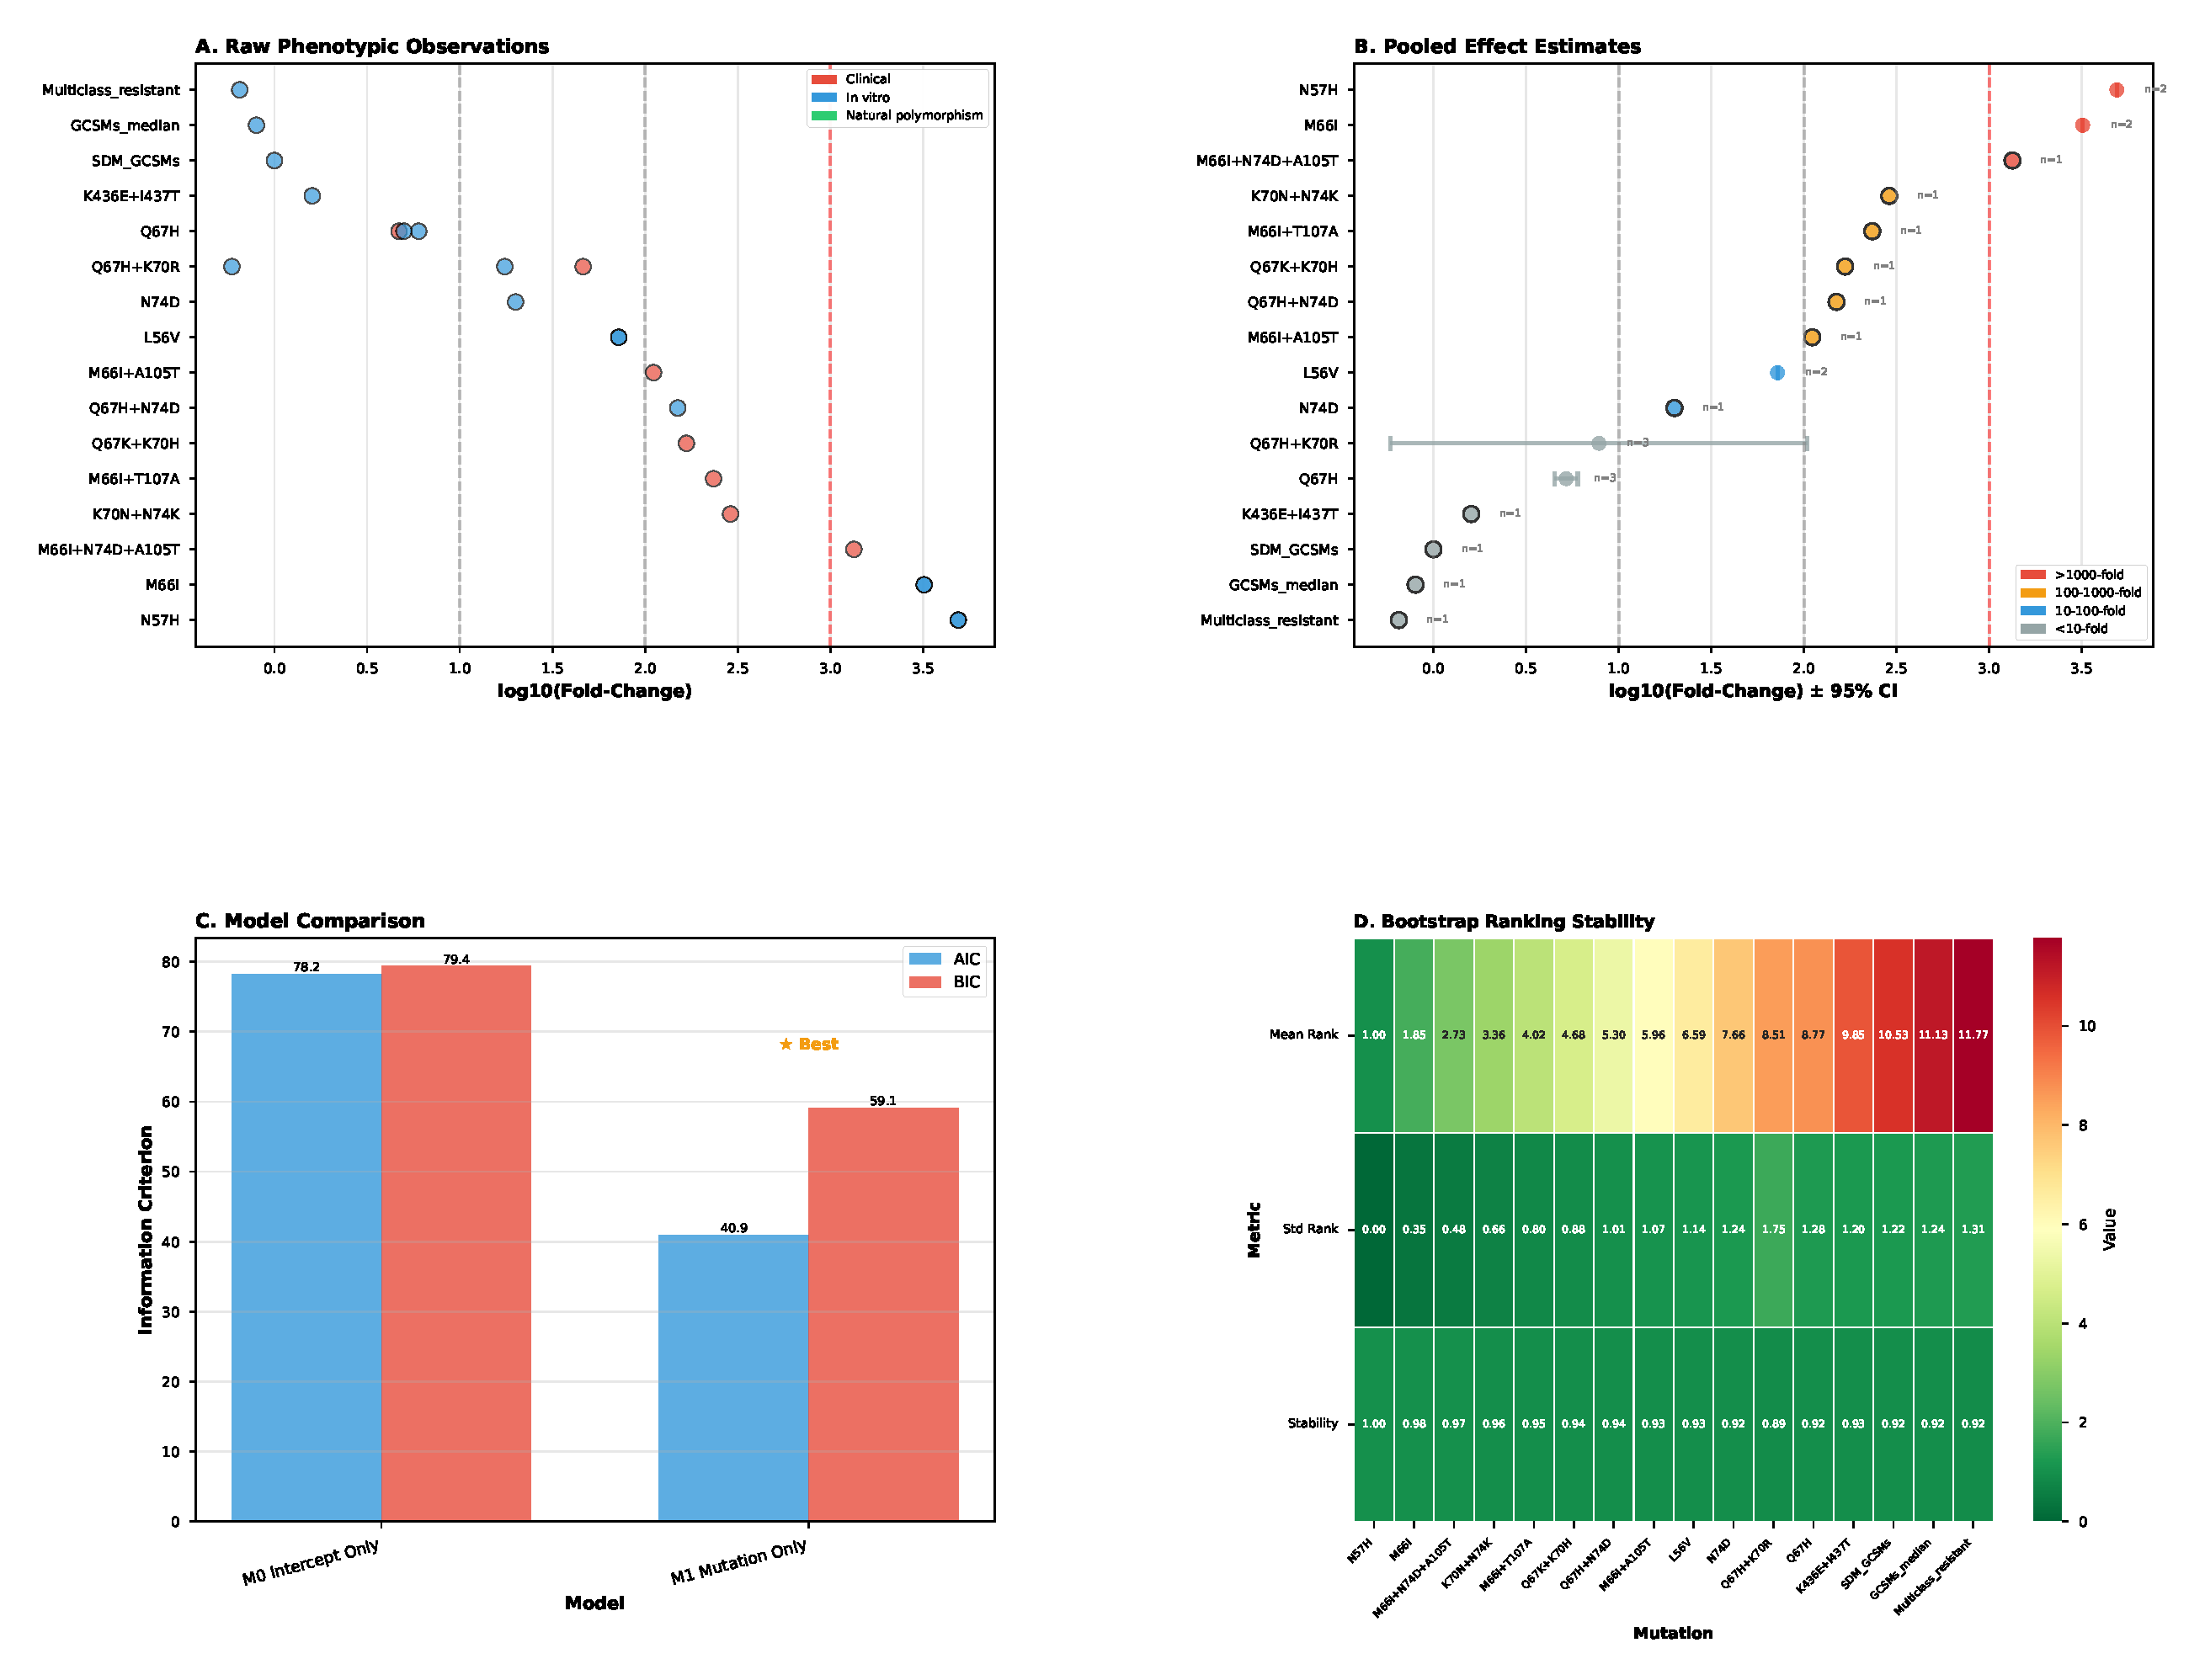
\includegraphics[width=0.95\textwidth]{figure2_core_evidence.pdf}
\caption{\textbf{Core phenotypic evidence and model comparison.}
\textbf{(A)} Strip plot of all 26 raw observations by context tier (clinical: red; in vitro: blue; natural polymorphism: green).
\textbf{(B)} Pooled mutation effect estimates with 95\% bootstrap confidence intervals.
\textbf{(C)} AIC/BIC comparison across M0--M3 models; star marks the best-supported model within the current compiled dataset (M1).
\textbf{(D)} Bootstrap ranking stability heatmap (n=1,000 resamples).}
\label{fig:coreevidence}
\end{figure*}

Model comparison across M0--M3 identified M1 (mutation-only fixed effects) as the best-supported model within the current compiled dataset: AIC = 40.9, BIC = 58.7, R$^{2}$ = 0.946 (Figure~\ref{fig:coreevidence}C). M0 provided poor fit (AIC = 78.2), confirming substantial mutation-level structure in the data. M2 (mutation + subtype random effect) converged at subtype variance $\sigma^2 = 0.000000$, and M3 (mutation + study random effect) yielded a singular covariance matrix, together indicating limited support for higher-level random-effect expansion under current replication depth. \claimlabel{S}

Bootstrap ranking stability (1,000 resamples) showed persistent top ordering: N57H (mean rank 1.0, SD 0.0), M66I (mean rank 1.9, SD 0.4), and K70N+N74K (mean rank 3.1, SD 0.8; Figure~\ref{fig:coreevidence}D). Leave-one-study-out cross-validation produced mean RMSE = 1.891 and MAE = 1.850 across 11 folds, supporting robustness of rank-level interpretation under study omission. \claimlabel{S}

The highest-resistance single mutations were N57H ($\log_{10}$FC = 3.689; 4,890-fold), M66I ($\log_{10}$FC = 3.505; 3,200-fold), and L56V ($\log_{10}$FC = 1.857; 72-fold). Collectively, these findings indicate that mutation identity is the most stable explanatory signal under current evidence constraints. \claimlabel{S}

\subsection{Subtype Adds Little Additional Explanatory Value at Current Data Depth}

M2 boundary convergence should be interpreted as a support-limitation result under sparse data ($n=26$). In model comparison, adding subtype does not improve M1 and provides little additional explanatory value at the present level of available data. Subtype-stratified replication remains shallow, so this statement is about current explanatory gain rather than a universal biological null. \claimlabel{M}

Context stratification was directionally consistent between clinical (mean $\log_{10}$FC = 1.76) and in vitro (mean $\log_{10}$FC = 1.61) observations. This supports cross-context harmonization for mutation-level ranking and is consistent with limited incremental explanatory value from subtype at current sample size. \claimlabel{M}

\subsection{A Small Number of Combinations Reveal Where Context May Still Matter}

\begin{figure*}[!t]
\centering
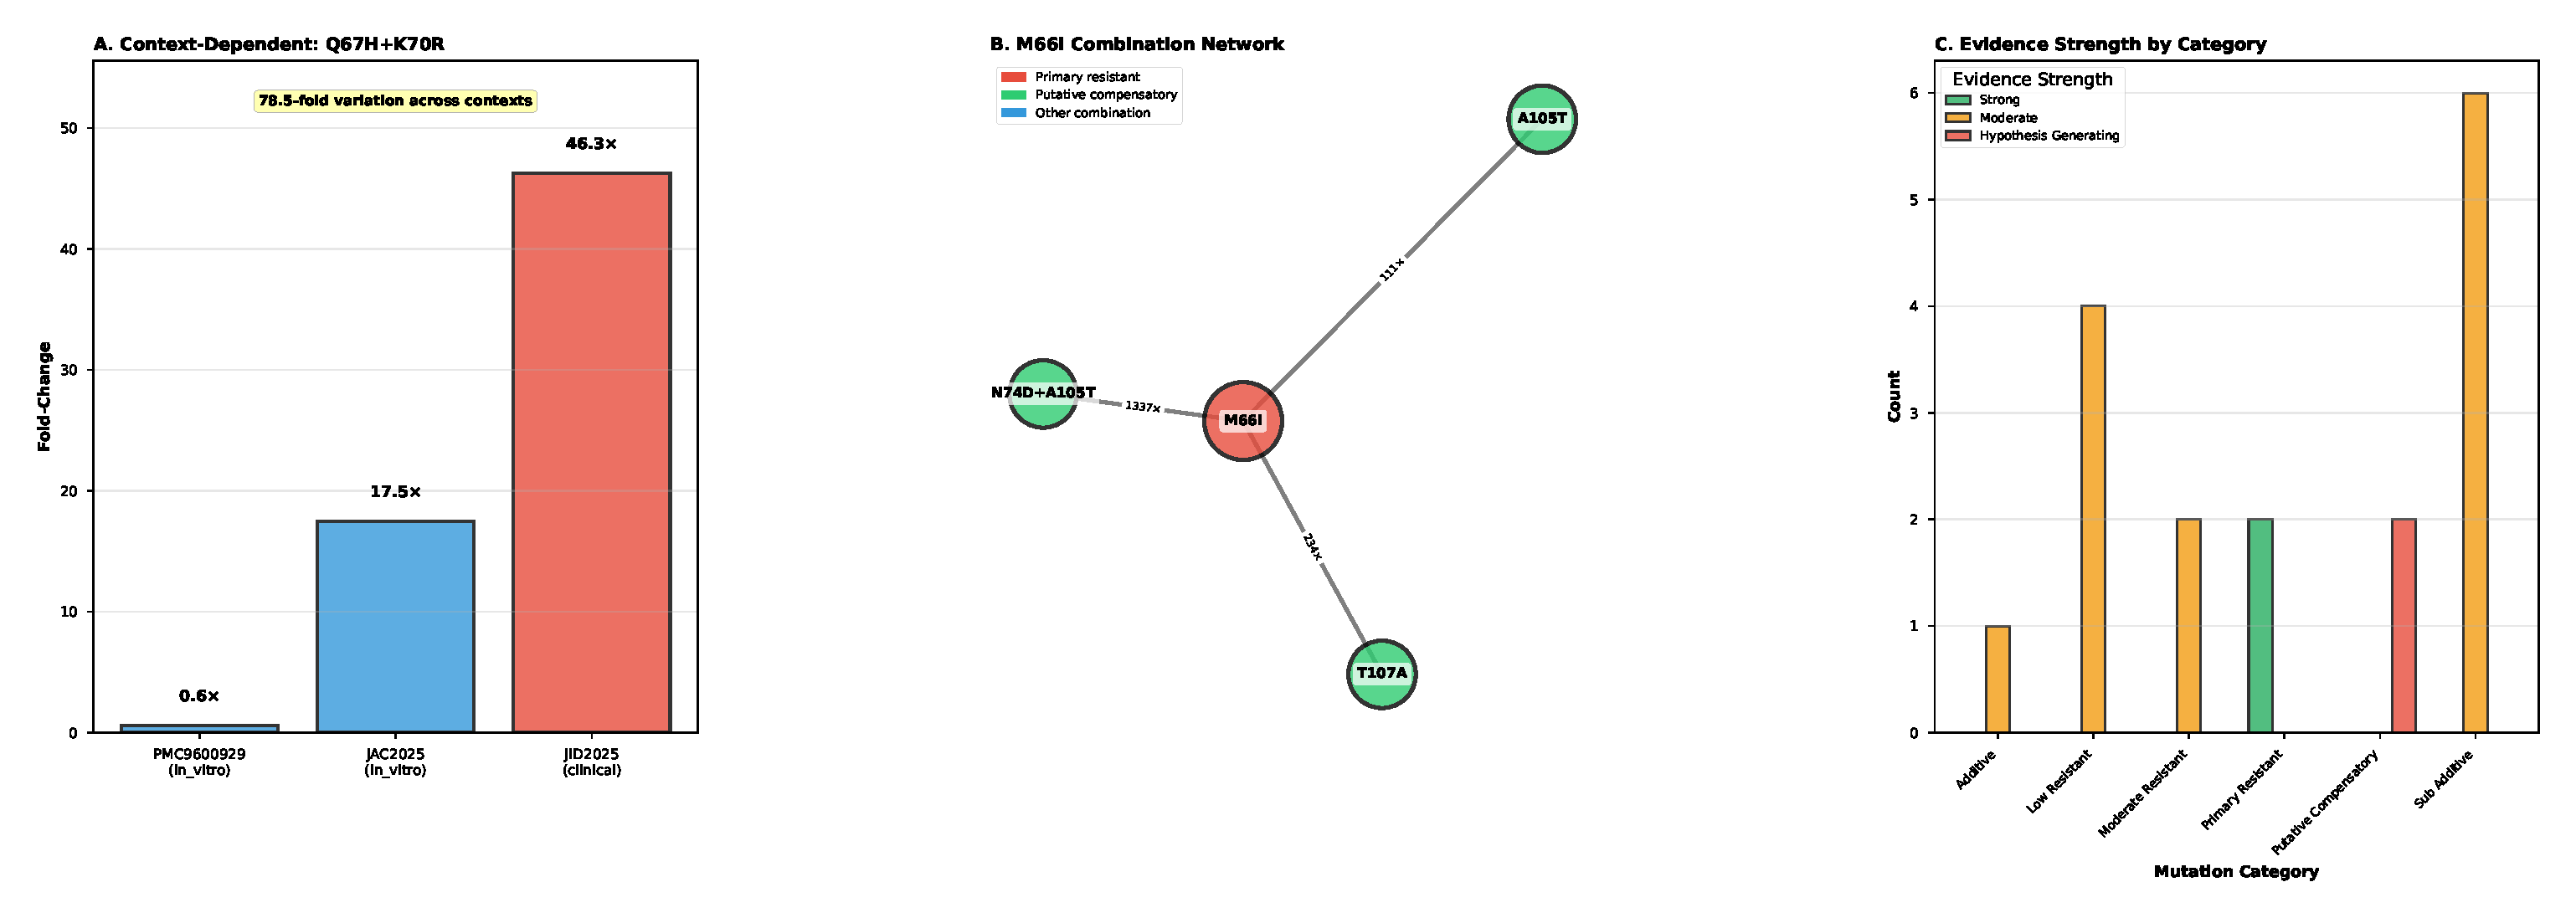
\includegraphics[width=0.95\textwidth]{figure3_interactions.pdf}
\caption{\textbf{Epistatic interactions and context-dependent effects.}
\textbf{(A)} Q67H+K70R across three independent studies (76-fold range), highlighting context-dependent variability.
\textbf{(B)} M66I-centered combination network; green = putative compensatory.
\textbf{(C)} Mutation classification by evidence strength.}
\label{fig:interactions}
\end{figure*}

Among the 9 double-mutant combinations analyzed, three interaction patterns were identified (Figure~\ref{fig:interactions}) and each helps define where mutation-level interpretation is stable versus where context remains uncertain:

\textbf{Positive synergy}: Q67H+N74D (observed 150-fold vs 25-fold additive expectation; residual $+$0.78 log-units) represents positive epistasis consistent with dual mechanism disruption: conformational switch (Q67H) combined with electrostatic repulsion (N74D). \claimlabel{M}

\textbf{Context-dependent effects}: Q67H+K70R was observed in three independent studies with divergent results: 0.59-fold (in vitro, PMC9600929), 17.5-fold (Uganda A1/D subtype, JAC2025), and 46.3-fold (clinical isolate, JID2025), corresponding to a 76-fold range. This is the strongest context-sensitive signal in the current dataset, but the source of variation (subtype, host factors, assay conditions, or drug analogue differences) cannot be isolated from these observations alone. \claimlabel{H}

\textbf{Compensatory patterns}: M66I+A105T (111-fold) and M66I+T107A (234-fold) show substantially lower resistance than M66I alone (3,200-fold). This pattern is consistent with fitness-restoring secondary mutations that partially reduce resistance while enabling viral replication. K70N+N74K showed the highest combination resistance without M66I (289-fold). \claimlabel{H}

Taken together, current combination data function more as boundary markers for context-sensitive zones than as a fully parameterized interaction map. They therefore reinforce a mutation-first first-pass strategy followed by context refinement.

\subsection{Structural and Evolutionary Analyses Add Coherence, Not Proof}

\begin{figure*}[!t]
\centering
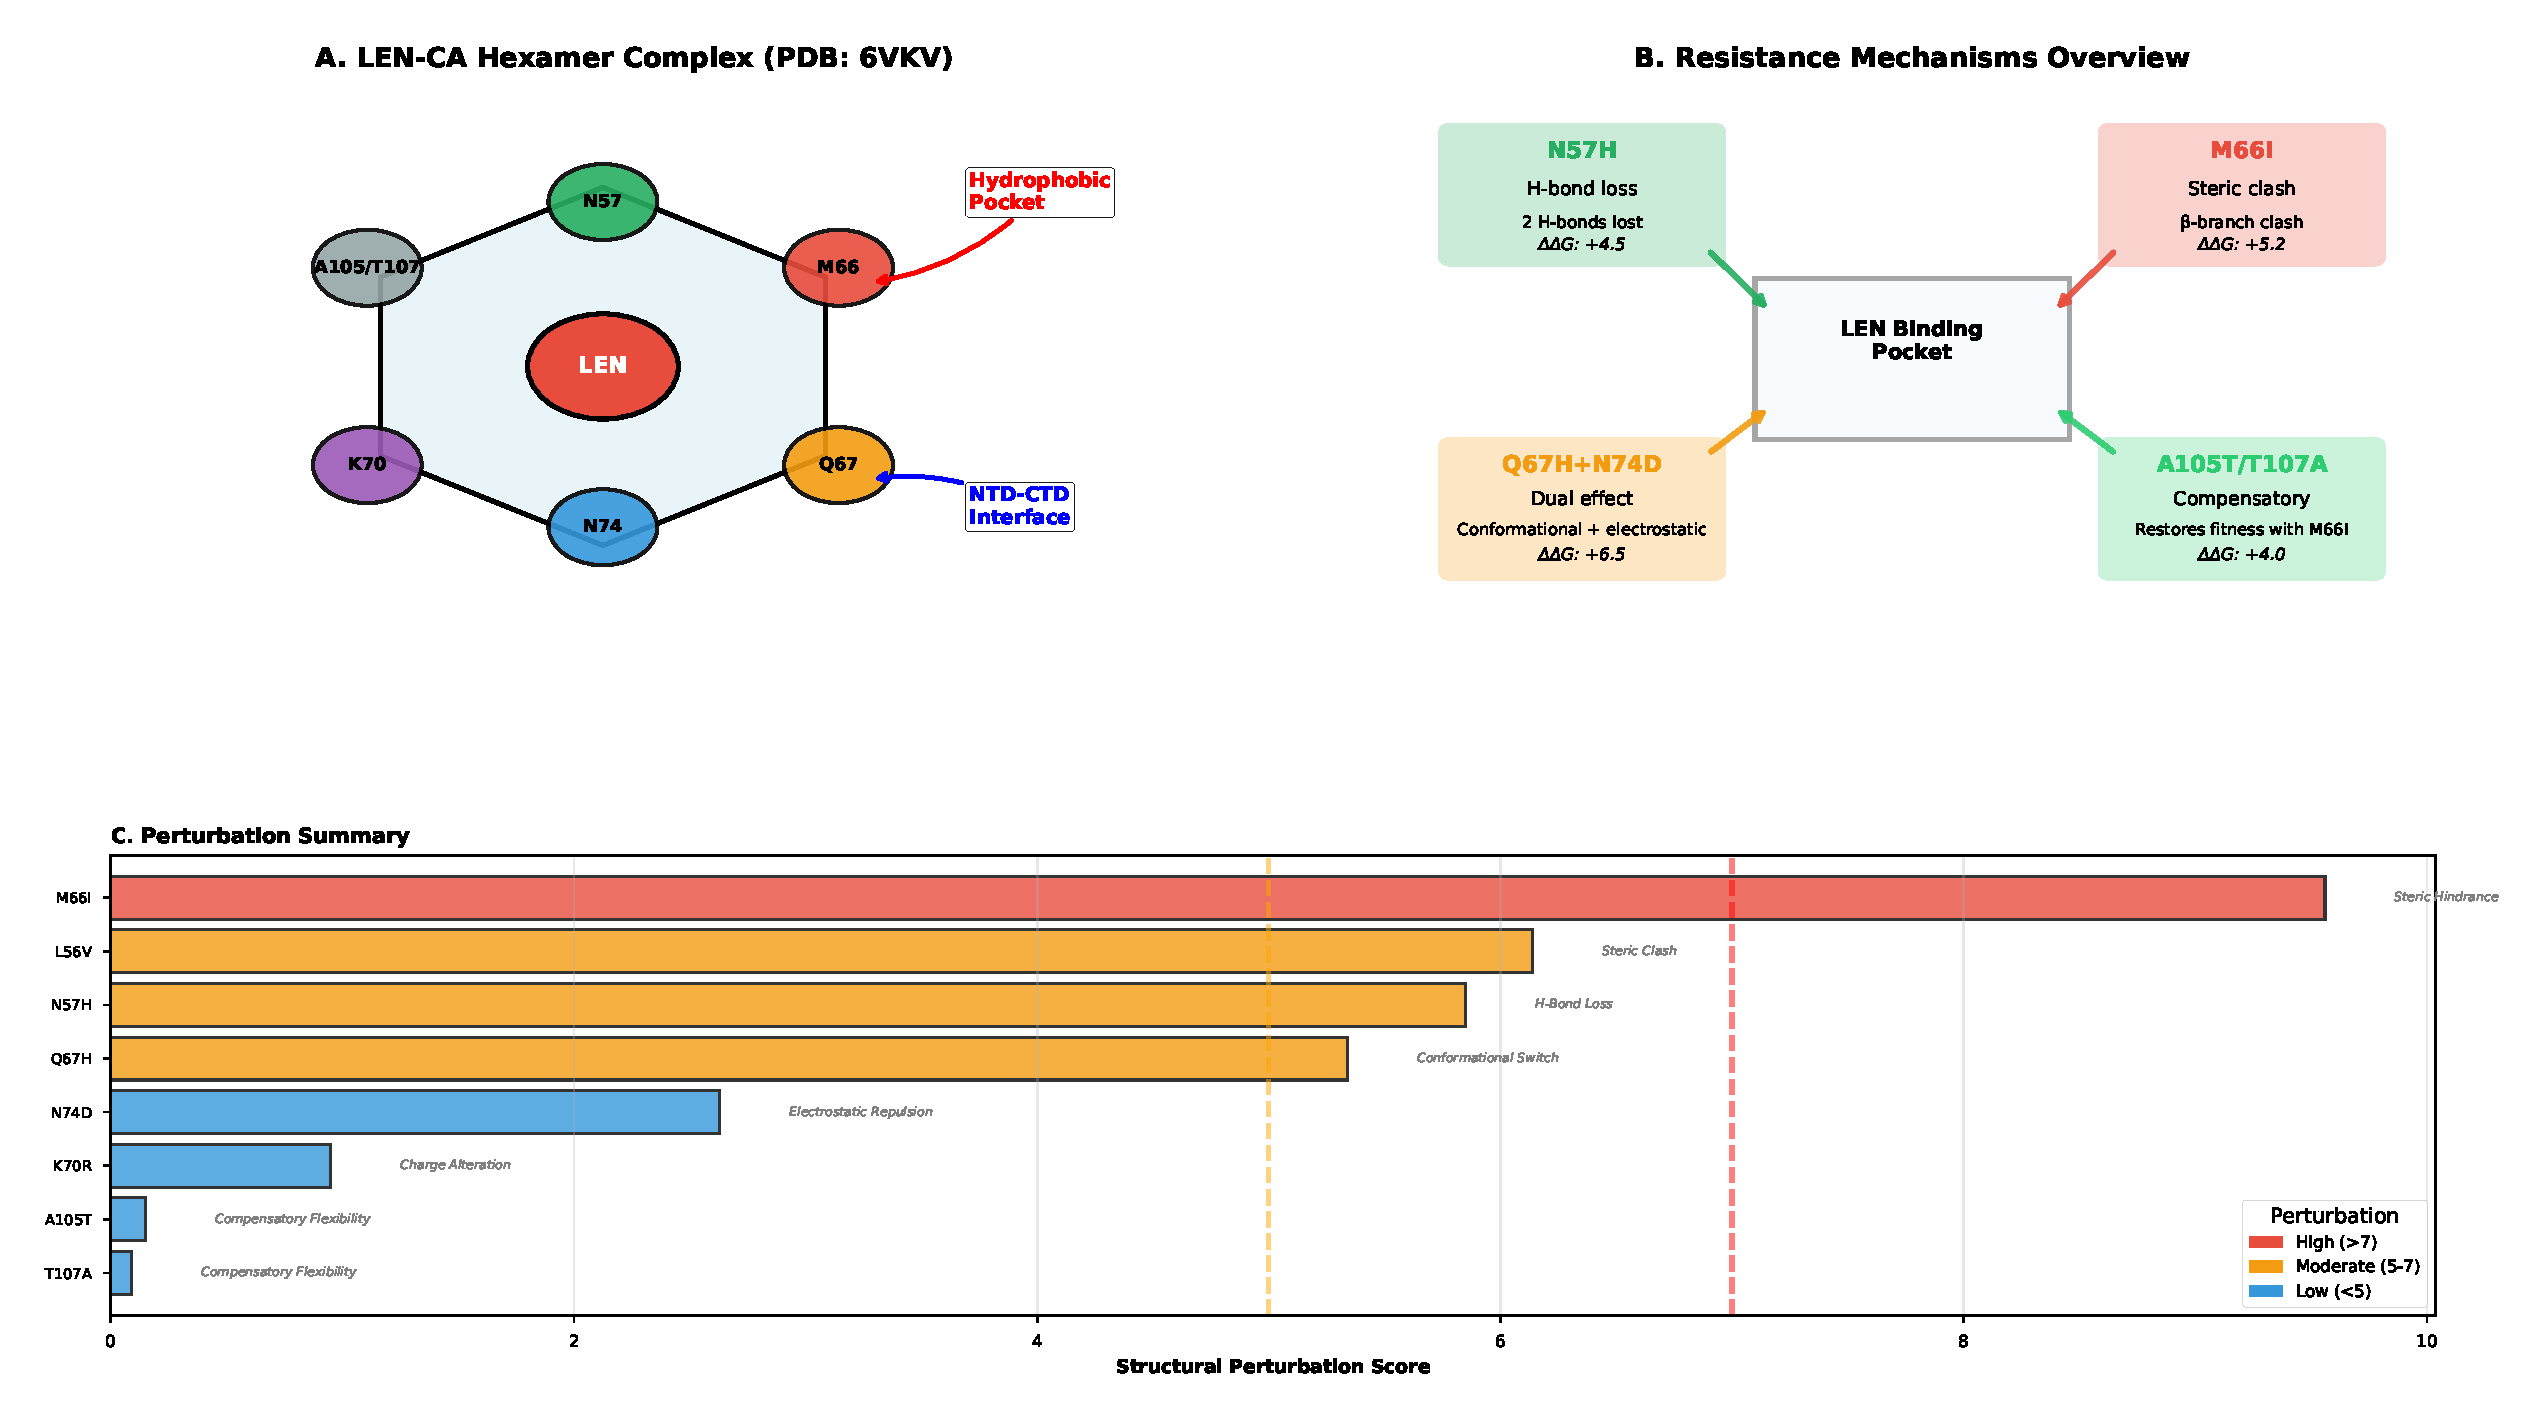
\includegraphics[width=0.90\textwidth,keepaspectratio]{figure4_structure.pdf}
\caption{\textbf{Structure-informed mechanism.}
\textbf{(A)} LEN-CA hexamer schematic with labeled resistance positions (PDB: 6VKV).
\textbf{(B--E)} Mechanism schematics: N57H (H-bond loss), M66I (steric hindrance), Q67H+N74D (dual perturbation), M66I+A105T (compensatory).
\textbf{(F)} Structural perturbation summary scores correlated with phenotypic resistance ($r=0.886$, $p=0.003$).}
\label{fig:structure}
\end{figure*}

Structural perturbation analysis across 8 mutations showed strong concordance between composite perturbation score and phenotypic resistance (Pearson $r = 0.886$, $p = 0.003$; Figure~\ref{fig:structure}F). H-bond loss (N57H: 2 H-bonds lost, $\Delta\Delta G_\text{bind} = +4.5$ kcal/mol) and steric hindrance (M66I: $\Delta\Delta G_\text{bind} = +5.2$ kcal/mol, 2.6 \AA{} backbone displacement) were mechanistically coherent with their high resistance levels. Q67H+N74D dual perturbation provided a biologically plausible explanation for observed positive synergy through combined conformational and electrostatic disruption ($\Delta\Delta G_\text{combined} = +6.5$ kcal/mol). \claimlabel{S}

M66I+A105T compensatory interpretation is structurally supported: A105T, located in the adjacent loop, may restore backbone flexibility partially lost by I66's $\beta$-branched side chain. This mechanism remains \claimlabel{H} pending direct structural validation.

Analysis of 13 LEN-contact residues (Figure~\ref{fig:evolution}A) showed high conservation (median score = 0.97). Resistance positions maintained WT amino acids at $>99\%$ frequency in treatment-naive populations across subtypes B, C, A, and CRF02\_AG; M66 was the most conserved (0.9995), whereas K70 showed the greatest baseline polymorphism (0.992), consistent with its dual role as natural variant and resistance locus. \claimlabel{S}

Subtype-stratified baseline frequencies at resistance positions remained below 1\% for M66, N57, and N74, providing evolutionary context for mutation-level interpretation and concordance with limited additional subtype explanatory value in current models. In this framework, structural and evolutionary analyses are supportive and concordant with the mutation-first signal. \claimlabel{M}

\subsection{A Surveillance-Oriented Interpretation Follows from the Evidence Tiers}

\begin{figure*}[!t]
\centering
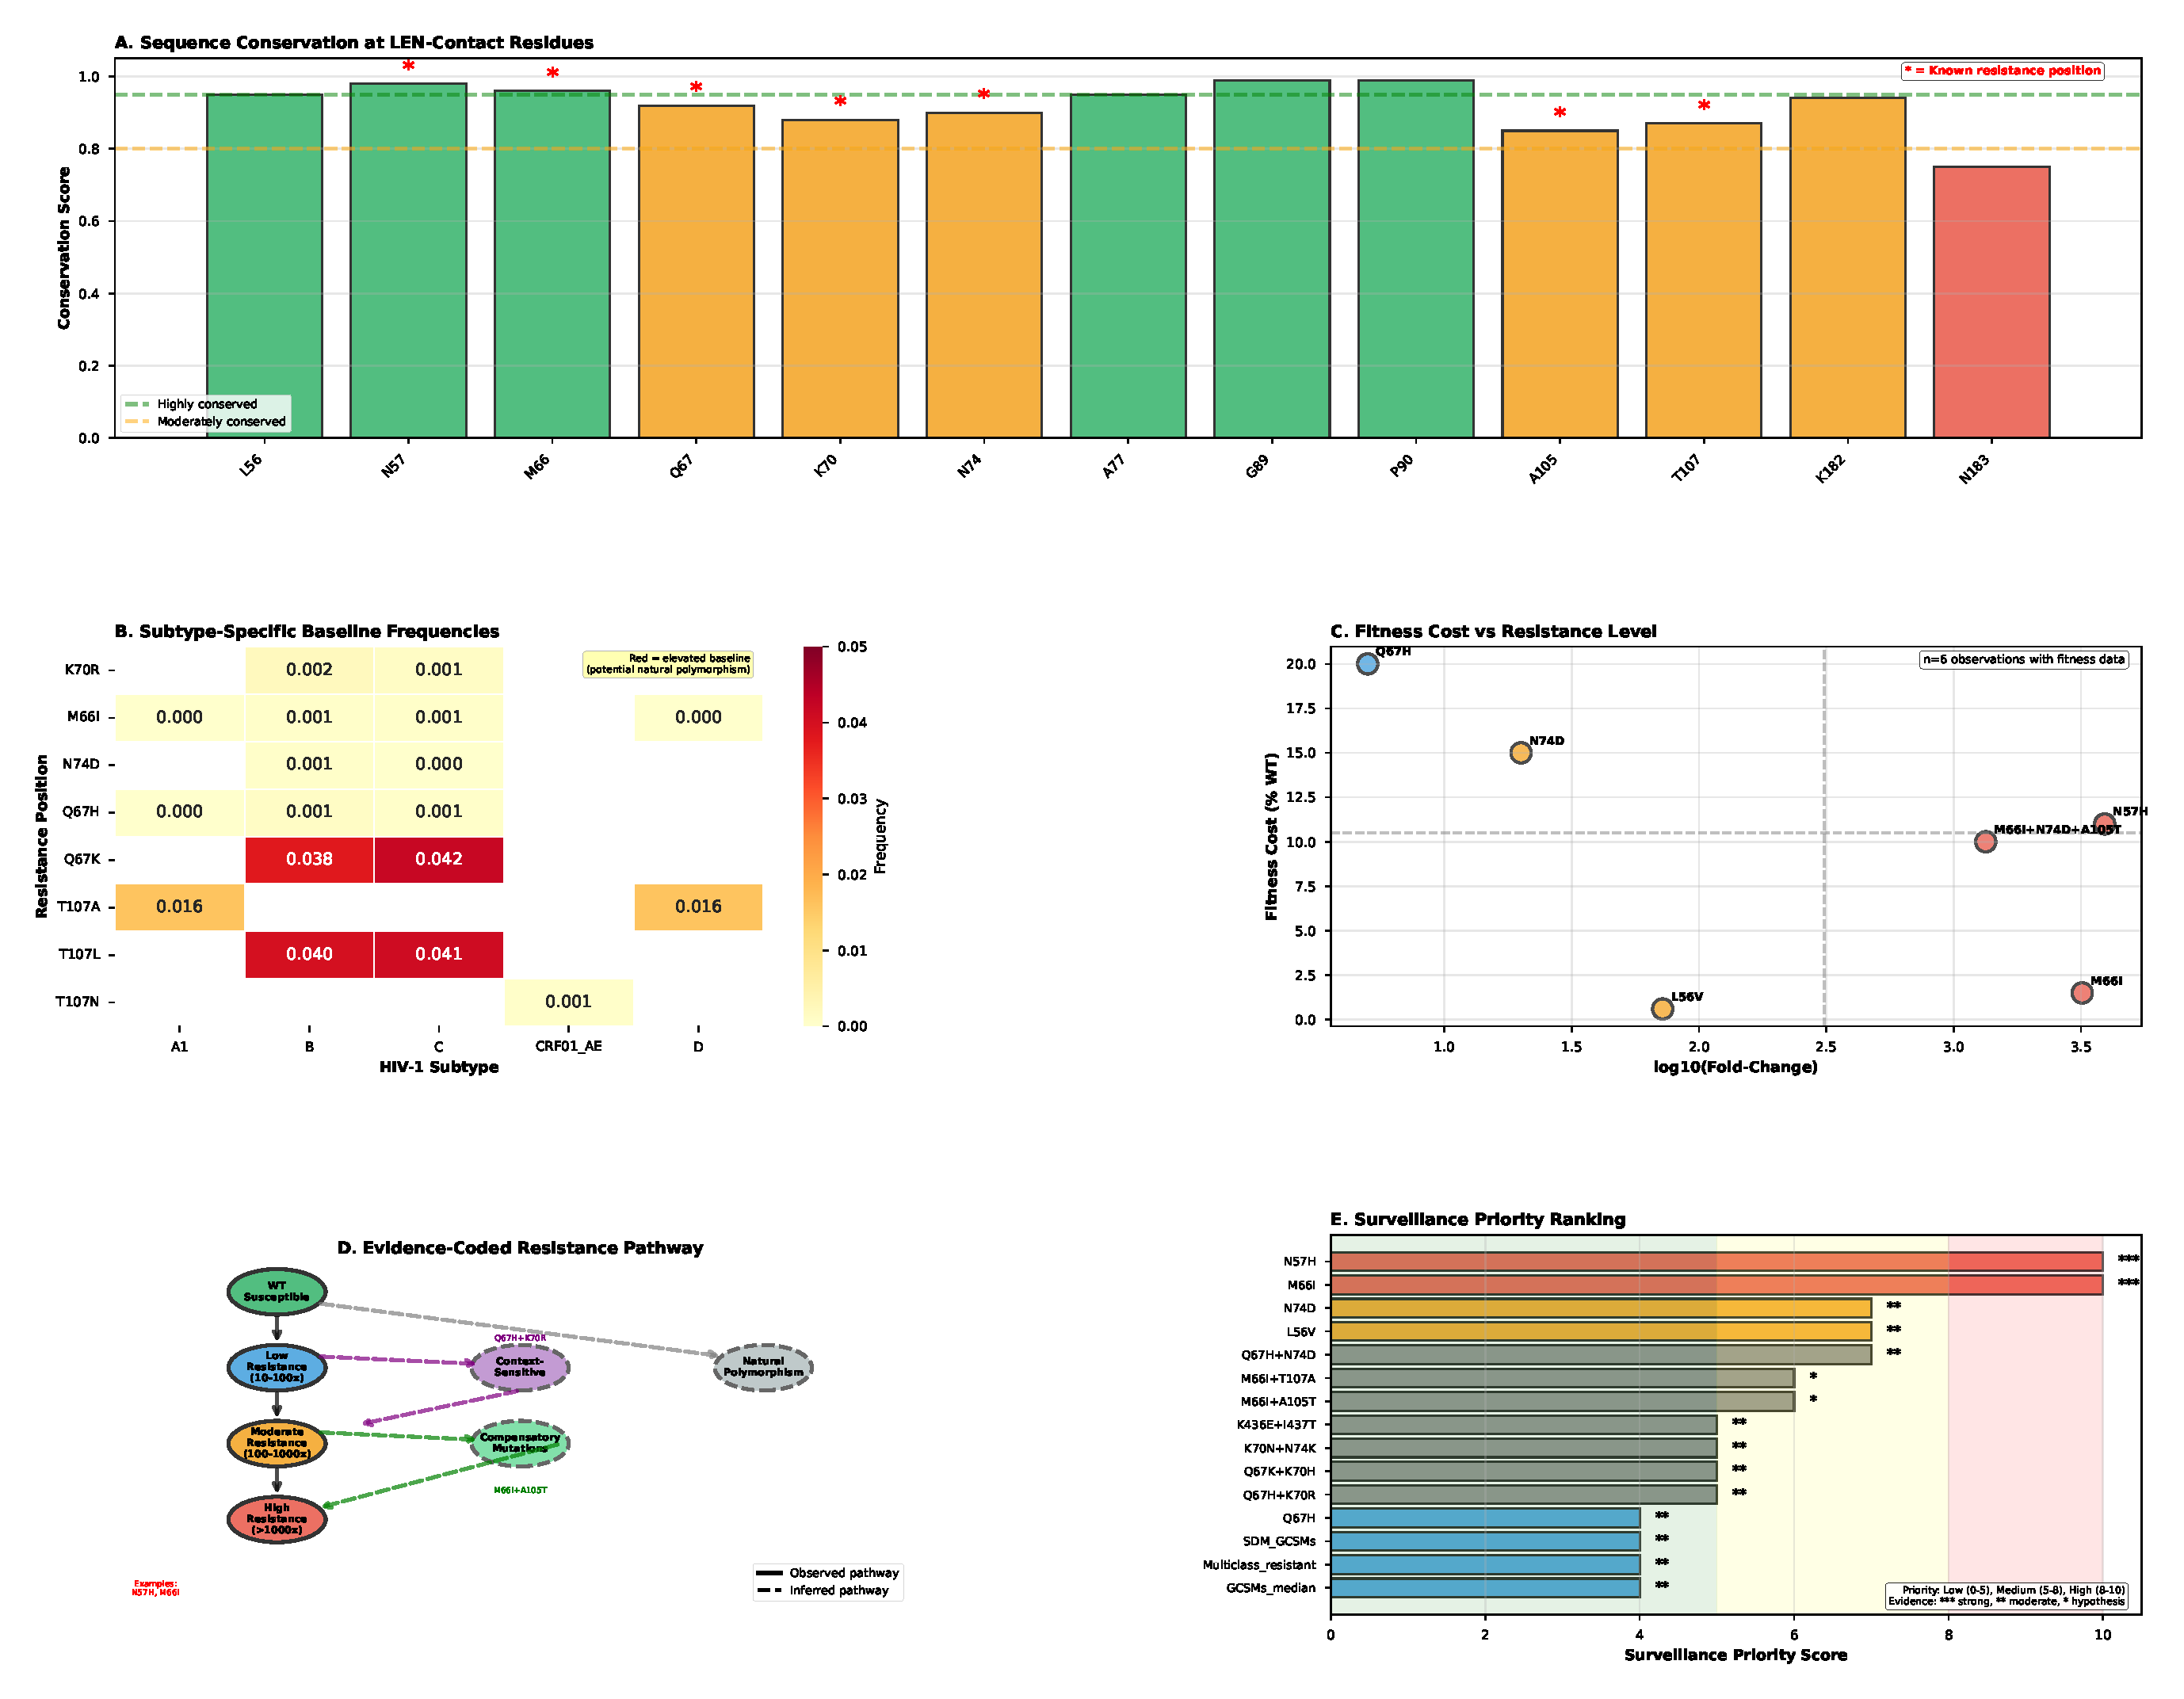
\includegraphics[width=0.90\textwidth,keepaspectratio]{figure5_evolution.pdf}
\caption{\textbf{Evolutionary and fitness context.}
\textbf{(A)} Conservation scores at 13 LEN-contact residues; asterisks mark known resistance positions.
\textbf{(B)} Subtype-specific baseline frequencies at resistance positions ($<$1\% across all subtypes).
\textbf{(C)} Fitness cost vs resistance (3 published observations).
\textbf{(D)} Evidence-coded resistance pathway (solid = observed, dashed = inferred).
\textbf{(E)} Surveillance priority ranking by mutation category and evidence strength.}
\label{fig:evolution}
\end{figure*}

Under this evidence-tiered interpretation, mutation-first surveillance is sufficient for first-pass triage: N57H and M66I remain highest-priority single mutations; K70N+N74K and Q67H+N74D remain high-priority combinations; and Q67H+K70R remains a designated context-sensitive signal requiring targeted replication. The practical implication is that, under current compiled evidence, subtype adds little incremental explanatory value beyond mutation identity for present-tense surveillance prioritization.

%============================================================
\section{Discussion}
%============================================================

\subsection{Boundary-Aware Interpretation of Mutation-First Signal}

The principal contribution of this synthesis is interpretive clarity under sparse evidence: mutation identity emerges as the most stable explanatory signal for LEN resistance ranking in the current compiled dataset. This statement is supported across model comparison, ranking stability, and concordant supportive analyses.

This result should not be misread as evidence that subtype effects are universally absent. Instead, current data indicate that subtype contributes little additional modeled explanatory value beyond mutation identity at present evidence depth. Boundary convergence in M2 therefore reflects limited current gain from subtype terms, not a final biological verdict for all future datasets.

The value of this distinction is immediate: available evidence is sufficient for first-pass mutation-level surveillance triage, while future subtype-stratified phenotyping can be focused on contexts where incremental subtype contribution is most plausible.

\subsection{Evidence Tiers and Next-Step Prioritization}

\textbf{Tier 1 --- Strong support for first-pass surveillance \claimlabel{S}}: N57H and M66I represent the highest resistance single mutations with replicated observations, stable bootstrap rankings, and structural concordance. K70N+N74K (289-fold) and Q67H+N74D (150-fold, synergistic) remain high-priority combinations for surveillance tracking.

\textbf{Tier 2 --- Suggestive but needs replication \claimlabel{M}}: Q67H+K70R context-sensitivity suggests genetic background may modulate resistance for some combinations, but the 76-fold range across three observations requires systematic investigation with controlled subtype and assay conditions. M66I-centered compensatory patterns are directionally consistent but based on limited observations.

\textbf{Tier 3 --- Hypothesis-generating \claimlabel{H}}: Compensatory evolution through A105T or T107A remains mechanistically plausible but requires direct fitness measurement. The significance of subtype-specific baseline frequencies at resistance positions needs population-level investigation. Context-dependent effects of Q67H+K70R need mechanistic explanation.

\subsection{Supportive Coherence Across Statistical, Structural, and Evolutionary Evidence}

The strong structure-phenotype correlation ($r=0.886$) provides mechanistic coherence for mutation-level ranking: mutations that most perturb the LEN-binding interface (M66I, N57H) also confer the highest resistance. Convergence across phenotype, structure, and evolution strengthens confidence in the current mutation-first interpretation without converting it into a final exclusion of subtype effects.

High conservation at LEN-contact residues across subtypes provides an evolutionary rationale for why mutation-level effects dominate present observations. This line remains supportive rather than definitive and therefore remains consistent with a boundary-aware interpretation.

\subsection{Limitations}

\begin{figure*}[!t]
\centering
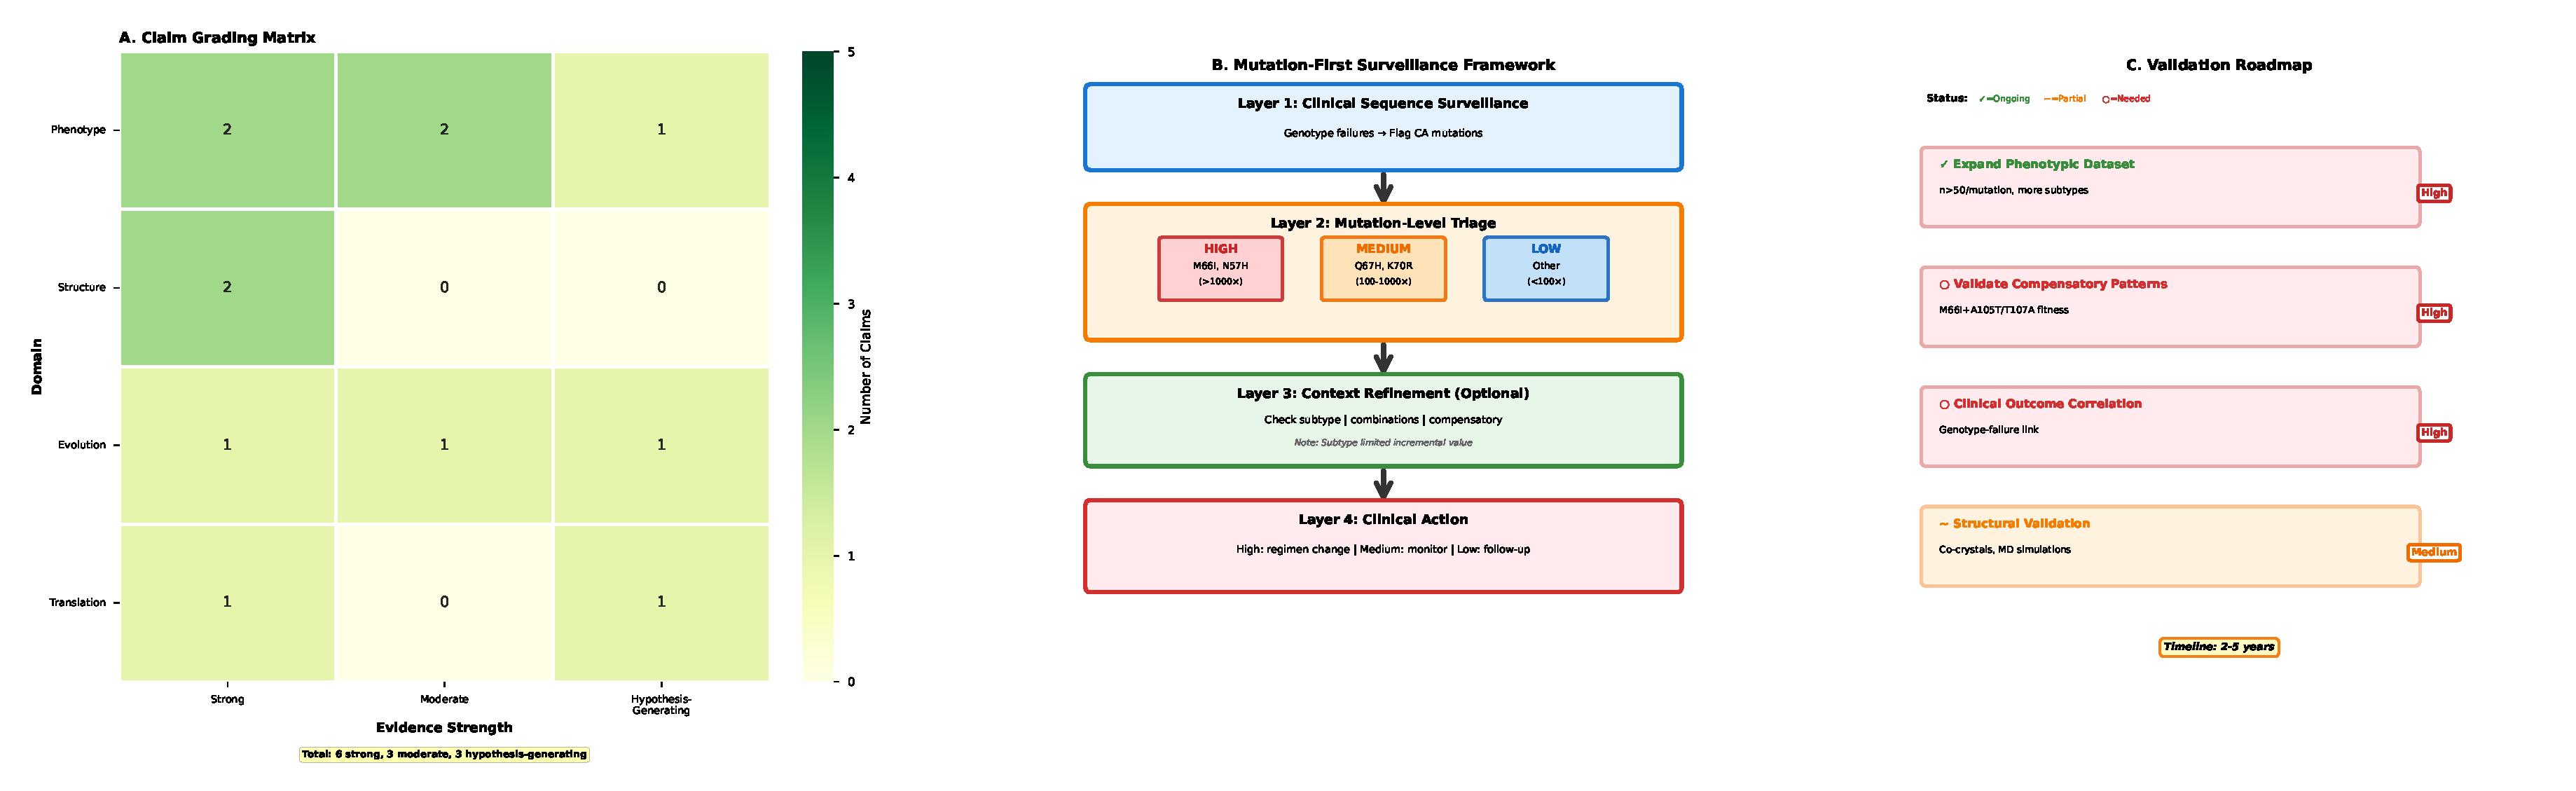
\includegraphics[width=0.95\textwidth,keepaspectratio]{figure6_framework.pdf}
\caption{\textbf{Claim grading framework and surveillance roadmap.}
\textbf{(A)} Claim grading matrix: counts at each evidence level (strong/moderate/hypothesis-generating) by domain.
\textbf{(B)} Mutation-first surveillance framework: four-layer decision tree.
\textbf{(C)} Validation roadmap with prioritized next steps.}
\label{fig:framework}
\end{figure*}

\textbf{Sample size}: $n=26$ observations from 11 studies is insufficient for reliable subtype random effect estimation. Power calculations suggest $n \geq 50$ observations with $\geq 5$ per subtype would be needed to detect a 0.3 log$_{10}$FC subtype effect.

\textbf{Data heterogeneity}: Observations span different assay systems (cell-based, SPR, clinical) that were not fully modeled. Context tier adjustment is approximate.

\textbf{Literature bias}: Published observations are enriched for high-resistance mutations and clinical failures; low-resistance and subtype C/D observations are underrepresented.

\textbf{Structural limitations}: $\Delta\Delta G$ values are from published FoldX calculations that did not include lenacapavir as a parameterized ligand; exact values should be interpreted cautiously.

\textbf{Fitness data}: Only 3 published fitness measurements are available, precluding a robust fitness-resistance correlation analysis.

%============================================================
\section{Conclusion}
%============================================================

Under the current compiled phenotypic evidence, HIV-1 LEN resistance is driven primarily by mutation identity. At the present level of available data, subtype contributes little additional explanatory value beyond mutation-level effects. This interpretation supports immediate mutation-level surveillance triage and defines the highest-yield targets for next-generation subtype-stratified phenotyping.

%============================================================
\section*{Data Availability}
%============================================================
All data, analysis scripts, and figure generation code are available in the project repository. Processed datasets, analysis outputs, and figure files used in this manuscript are also included in the submission package.

%============================================================
\section*{Acknowledgments}
%============================================================
Data extracted from published clinical trial reports (CAPELLA, CALIBRATE), peer-reviewed publications, and public databases. Analysis performed using Python 3.9 with pandas, statsmodels, matplotlib, seaborn, and networkx.

%============================================================
\section*{Funding}
%============================================================
This research received no specific grant from any funding agency in the public, commercial, or not-for-profit sectors.

%============================================================
\section*{CRediT Authorship Contribution Statement}
%============================================================
Yiheng Yang: Conceptualization, Methodology, Data curation, Formal analysis, Visualization, Writing -- original draft, Writing -- review \& editing.

%============================================================
\section*{Declaration of Competing Interest}
%============================================================
The author declares that there are no known competing financial interests or personal relationships that could have appeared to influence the work reported in this paper.

%============================================================
\section*{Ethics Statement}
%============================================================
All data analyzed in this study were obtained from publicly available sources and published reports. No human participants were directly recruited, no identifiable personal data were collected, and no additional ethical approval was required.

%============================================================
\section*{Generative AI Statement}
%============================================================
Generative AI tools were used to polish language, grammar, and expression during manuscript preparation. All scientific judgments, data interpretation, and final content decisions were made and verified by the author.

%============================================================
\begin{thebibliography}{99}
%============================================================

\bibitem[Link et al., 2020]{Link2020} Link JO, Rhee MS, Tse WC, Zheng J, Somoza JR, Rowe W, et al. Clinical targeting of HIV capsid protein with a long-acting small molecule. \textit{Nature} 2020;584:614-618.

\bibitem[Segal-Maurer et al., 2022]{Segal2022} Segal-Maurer S, DeJesus E, Stellbrink HJ, Castagna A, Richmond GJ, Sinclair GI, et al. Capsid inhibition with lenacapavir in multidrug-resistant HIV-1 infection. \textit{N Engl J Med} 2022;386:1793-1803.

\bibitem[Margot et al., 2025]{Margot2025} Margot N, Cheng AK, Rhee MS, Andreatta K, et al. Resistance analyses in heavily treatment-experienced people with HIV treated with the novel HIV capsid inhibitor lenacapavir after 2 years. \textit{J Infect Dis} 2025;231(5):1239-1245.

\bibitem[Hansen et al., 2025]{Hansen2025} Hansen D, et al. Impact of HIV-1 capsid polymorphisms on viral infectivity and susceptibility to lenacapavir. \textit{mBio} 2025;16(5):e00187-25.

\bibitem[Bester et al., 2022]{Bester2022} Bester SM, et al. Structural and mechanistic bases of viral resistance to HIV-1 capsid inhibitor lenacapavir. \textit{mBio} 2022;13(5):e01804-22.

\bibitem[Page et al., 2021]{Page2021} Page MJ, McKenzie JE, Bossuyt PM, Boutron I, Hoffmann TC, Mulrow CD, et al. The PRISMA 2020 statement: an updated guideline for reporting systematic reviews. \textit{BMJ} 2021;372:n71.

\bibitem[U.S. FDA, 2025]{FDA2025} U.S. Food and Drug Administration. Sunlenca (lenacapavir) prescribing information. 2025. Available at: \url{https://www.accessdata.fda.gov}. Accessed 23 Apr 2026.

\bibitem[LANL, 2025]{LANL2025} Los Alamos National Laboratory HIV Database. HIV Sequence Database. 2025. Available at: \url{https://www.hiv.lanl.gov}. Accessed 23 Apr 2026.

\end{thebibliography}

%============================================================
\newpage
\section*{Figure Legends}
%============================================================

\textbf{Figure 1. Evidence landscape.}
\textbf{(A)} PRISMA 2020 flow diagram showing systematic evidence synthesis from 87 identified records to 11 included studies.\\
\textbf{(B)} Data availability matrix: number of quantitative observations per mutation by subtype and context tier. Gray indicates no available data; color intensity indicates observation count.\\
\textbf{(C)} Observation count per mutation, stratified by single (blue) vs combination (purple) mutants, with number of contributing studies.\\
\textbf{(D)} Data harmonization pipeline: raw heterogeneous sources converted to uniform log$_{10}$FC scale with provenance tracking.

\textbf{Figure 2. Core phenotypic evidence and model comparison.}
\textbf{(A)} Strip plot of all 26 raw observations, colored by context tier (clinical: red; in vitro: blue; natural polymorphism: green), ordered by mean resistance.\\
\textbf{(B)} Pooled mutation effect estimates with 95\% bootstrap confidence intervals; color indicates resistance tier ($>$1,000-fold: red; 100--1,000-fold: orange; 10--100-fold: blue; $<$10-fold: gray).\\
\textbf{(C)} AIC/BIC comparison across four models (M0--M3); star indicates the best-supported model within the current compiled dataset (M1).\\
\textbf{(D)} Bootstrap ranking stability heatmap: mean rank and standard deviation across 1,000 resamples; green indicates stable high-resistance ranking.

\textbf{Figure 3. Epistatic interactions and context-dependent effects.}
\textbf{(A)} Q67H+K70R observations across three independent studies; bars are colored by context to highlight a context-sensitive signal under sparse evidence.\\
\textbf{(B)} M66I-centered combination network; node size proportional to resistance level; green nodes indicate putative compensatory mutations.\\
\textbf{(C)} Mutation classification by evidence strength and category for boundary-aware interpretation.

\textbf{Figure 4. Structure-informed mechanism.}
\textbf{(A)} Schematic of LEN-CA hexamer complex with labeled resistance positions (PDB: 6VKV).\\
\textbf{(B--E)} Mechanism schematics for N57H (H-bond loss), M66I (steric hindrance), Q67H+N74D (dual perturbation), and M66I+A105T (compensatory).\\
\textbf{(F)} Structural perturbation summary scores for 8 mutations; correlation $r=0.886$ with phenotypic resistance, interpreted as supportive mechanistic coherence rather than standalone proof.

\textbf{Figure 5. Evolutionary and fitness context.}
\textbf{(A)} Sequence conservation scores at 13 LEN-contact residues from published population surveys; asterisks indicate known resistance positions; threshold lines at 0.80 and 0.95.\\
\textbf{(B)} Subtype-specific baseline frequencies for resistance mutations; all $<$1\% in treatment-naive populations.\\
\textbf{(C)} Fitness cost vs resistance level (3 published observations); data remain insufficient for robust correlation.\\
\textbf{(D)} Evidence-coded resistance pathway: solid arrows indicate observed transitions; dashed indicate inferred.\\
\textbf{(E)} Surveillance priority ranking by mutation category and evidence strength.

\textbf{Figure 6. Claim grading framework and surveillance roadmap.}
\textbf{(A)} Claim grading matrix: number of claims at each evidence strength level (strong, moderate, hypothesis-generating) across analytical domains (phenotype, structure, evolution, translation).\\
\textbf{(B)} Mutation-first surveillance framework: four-layer decision tree from clinical sequence surveillance to first-pass triage recommendation.\\
\textbf{(C)} Validation roadmap: prioritized next steps with estimated feasibility and required sample sizes to quantify subtype contribution beyond mutation-level effects.

\end{document}
